% LEXITAX AUDIT manuscript -- DRAFT FOR AUTHOR REVIEW (not submission-ready; not submitted).
% tables/*.tex and figures/test_outcomes.pdf are generated from the committed experiment results (TEST run
% 20261127T104925Z-0f293784) and must not be edited by hand; the generator, the claim-to-evidence audit and the
% author questionnaire are kept in the project repository (research_paper/manuscript/).
% Target venue not yet selected: generic IEEEtran conference template.
\documentclass[conference]{IEEEtran}
\usepackage[T1]{fontenc}
\usepackage{cite}
\usepackage{amsmath}
\usepackage{graphicx}
\usepackage{booktabs}
\usepackage{url}
\usepackage[hidelinks]{hyperref}
\def\BibTeX{{\rm B\kern-.05em{\sc i\kern-.025em b}\kern-.08em
    T\kern-.1667em\lower.7ex\hbox{E}\kern-.125em X}}
% Start a new row of author blocks (IEEEtran author alignment environment; no manual spacing).
\makeatletter
\newcommand{\linebreakand}{%
  \end{@IEEEauthorhalign}
  \hfill\mbox{}\par
  \mbox{}\hfill\begin{@IEEEauthorhalign}
}
\makeatother

\begin{document}

\title{Silent Errors versus Safe Abstention in Staged Customs Pre-Assessment: An Empirical Study of Product and Jurisdiction Resolution}

% Two-column, two-row author layout: \and separates blocks in a row; \linebreakand starts a new row.
\author{
\IEEEauthorblockN{Syeda Sayeeda Farhath}
\IEEEauthorblockA{Department of Computer Science and Engineering\\
Vardhaman College of Engineering\\
Hyderabad, India\\
syedasayeedafarhath@ieee.org}
\and
\IEEEauthorblockN{Siddharth Karanam}
\IEEEauthorblockA{Department of Computer Science and Engineering\\
Vardhaman College of Engineering\\
Hyderabad, India\\
siddharthreddy1908@gmail.com}
\linebreakand
\IEEEauthorblockN{P.\ Naga Bhargav Reddy}
\IEEEauthorblockA{Department of Computer Science and Engineering\\
Vardhaman College of Engineering\\
Hyderabad, India\\
nagabhargavreddy175@gmail.com}
\and
\IEEEauthorblockN{Baalne Anjali}
\IEEEauthorblockA{Department of Computer Science and Engineering\\
Vardhaman College of Engineering\\
Hyderabad, India\\
anjali1820@vardhaman.org}
}

\maketitle

\begin{abstract}
Assistive customs pre-assessment tools map a free-text product description and a destination to a tariff
classification, duty, value-added tax (VAT) and a landed cost. When such a tool cannot resolve an input, it can either
answer anyway or abstain. We study this choice in an existing staged prototype, comparing a single-step baseline (B),
the original fixed six-stage Python pipeline (S0) and a corrected pipeline (S1) that resolves products through explicit
evidence tiers, identifies destinations against ISO~3166-1, and refuses instead of substituting default rates. A
benchmark with labels independent of the systems (529 product and 1{,}465 country items scored in a group-held-out TEST
split) was frozen before evaluation; S1's three parameters were tuned on DEV only, and TEST was run once. On held-out
TEST, S1 made no silent product errors (0/359; 95\% cluster-bootstrap interval [0, 0]) while answering 68.8\% of items,
whereas S0 answered every item and was silently wrong on 44.3\% [38.2, 51.2]. No system reliably identified held-out
country forms: none identified typographical variants, and S0 correctly identified only three localised-name items while
also producing 12 silent identification errors. S1's safety on these forms comes from abstention. For tax-data behaviour, B and
S0 computed costs with wrong, mostly default, rates for nearly every held-out item, while S1 refused all of them,
including 137 items for which tax data existed. Product errors never changed computed costs, because the prototype's tax
table is keyed by country only; country errors did. The data are synthetic and the results do not establish legal
classification validity.
\end{abstract}

\begin{IEEEkeywords}
selective prediction, abstention, silent errors, customs pre-assessment, Harmonized System, entity resolution, error
propagation
\end{IEEEkeywords}

\section{Introduction}
Customs pre-assessment applications help traders estimate the duty and tax due on a shipment before declaration. In a
typical staged design, a product description is mapped to a Harmonized System (HS) code~\cite{wcohs2022}, the
destination is mapped to a jurisdiction, rates are looked up, and a landed cost is computed. Each stage can fail. The
practically important question is not only how often a stage is wrong, but whether the error is \emph{visible}: an
explicit ``cannot resolve'' is recoverable by a human, whereas a fabricated code or a silently substituted default rate
propagates into a plausible-looking number.

This paper studies that distinction empirically in LEXITAX AUDIT, an assistive prototype whose original implementation
resolves products and destinations permissively and falls back to defaults. We ask: \emph{how do product-identification
and destination-resolution approaches trade coverage against silent (unflagged) errors, and how do those errors
propagate into duty, VAT and landed-cost outputs?} We compare three systems on a benchmark whose labels come from
reference data and pre-declared rules, never from system outputs, and we evaluate the held-out split once, after freezing
data, code, configuration and the tuning record.

Our contributions are: (i) a reproducible benchmark and evaluation protocol for product and jurisdiction resolution in
this setting, with cluster-level statistics; (ii) a three-system comparison of silent errors, coverage and abstention on
a held-out split; (iii) an error-propagation analysis separating product from jurisdiction errors; and (iv) a corrected
pipeline (S1) whose behaviour, including its failures, is reported in full. The systems are fixed sequential Python
pipelines; none uses a large language model (LLM) or autonomous agents, and the stage names inherited from the prototype
(e.g.\ ``agent'') do not denote agents in the sense of~\cite{wooldridge1995}.

\section{Related Work}
The trade-off between error and rejection was formalised by
Chow~\cite{chow1970}; selective classification studies the resulting risk--coverage trade-off~\cite{elyaniv2010,
geifman2017}, and abstention has been studied for question answering under domain shift~\cite{kamath2020} and across
natural language processing tasks~\cite{xin2021}. These works typically derive abstention from model confidence. S1 has
no confidence score; it abstains on explicit, rule-defined evidence conditions, and we report coverage and silent-error
rate in the same spirit.

Mapping noisy descriptions and place names to canonical records is
a record-linkage problem~\cite{fellegi1969, elmagarmid2007, christen2012}. S1's bounded typo tolerance uses an
edit-distance criterion in the tradition of~\cite{damerau1964, navarro2001}.

Automatic HS-code assignment has been approached with
text-categorisation methods~\cite{ding2015} and, recently, with LLMs~\cite{koch2025}; a 2026 review surveys machine-learning,
deep-learning and LLM-based HS classification~\cite{wube2026}. Machine learning is also used for customs fraud
detection~\cite{kim2020date}, and the World Customs Organization has discussed data mobilisation in
customs~\cite{mikuriya2020}. Our study does not propose a classifier; it evaluates whether a pre-assessment pipeline
answers or abstains when resolution fails, and what the downstream financial consequence is.

Errors in early pipeline stages cascade into later
ones~\cite{finkel2006}, and production ML systems accumulate hidden failure modes~\cite{sculley2015, breck2017}. We use
perturbation-style test categories in the spirit of behavioural testing~\cite{ribeiro2020}, and guard against
leakage~\cite{kapoor2023} with a frozen, group-held-out TEST split. Policy lookup in the prototype uses TF-IDF
weighting~\cite{salton1988}; its retrieval quality is not evaluated here.

\section{Systems and Problem Formulation}
\subsection{Problem Formulation}
An input consists of a product description, a destination string, price, quantity and shipping cost. A
system either returns an HS-6 code, a jurisdiction, duty and VAT rates and a landed cost (customs value = price
$\times$ quantity + shipping; duty and VAT are applied to it in sequence), or it abstains or refuses at some stage. For a
product description the gold decision is either an HS-6 code (\emph{answer}) or \emph{decline}; for a destination it is
an ISO~3166-1 country~\cite{iso3166} or ``no country'', together with whether the project's tax table holds rates for that
country (\emph{compute} or \emph{refuse}).

\subsection{Compared Systems}
The baseline B is a single function: the product matches if the input is a substring of a catalogue name (otherwise
the HS code is shown as ``N/A''); the destination must equal a tax-table name exactly, otherwise default rates of 5\% duty
and 10\% VAT are applied silently.

The original pipeline S0 consists of six fixed, sequential functions (input, product, policy lookup, tax,
calculation, report) sharing a dictionary. Product resolution uses substring and token-overlap matching and falls back
to a fabricated HS code; destination matching accepts partial substrings in both directions and otherwise applies the
same defaults; a missing exchange rate is replaced by 1.0.

The corrected pipeline S1 has six fixed stages: input validation, jurisdiction resolution, tax-data availability,
product resolution, landed-cost calculation (reusing S0's arithmetic) and policy lookup. Jurisdiction resolution uses an
alias table built from ISO~3166-1 codes and names (via the pycountry package) plus the tax table's own names, and keeps
\emph{identification} separate from \emph{tax-data availability}: an identified country without rates is refused, never
defaulted. Product resolution uses three deterministic evidence tiers: T1, exact normalised name; T2, whole-token
containment of a catalogue base-type name, with maximality, uniqueness of the implied HS code and an evidence-coverage
threshold; T3, T2 with a bounded number of typo edits on sufficiently long tokens. Otherwise S1 abstains and states why.
Costs are computed only when both the product and the jurisdiction are resolved. S1 has three tunable product
parameters (coverage threshold, maximum typo edits, minimum token length for typo matching).

\section{Experimental Methodology}
\subsection{Benchmark Data}
The prototype's own tables are synthetic: a catalogue of 1{,}200 product names (60 base types $\times$ 20
name variants, 43 HS-6 codes), a tax table for 40 jurisdictions with unsourced rates, and placeholder policy records.
Benchmark items were generated by pre-declared rules from reference data (Table~\ref{tab:bench}). Product categories
P1--P7 cover exact names, formatting variants, typos, under-specified short forms, confusable neighbours, ambiguous words
and out-of-catalogue items; P7 uses Unicode emoji names~\cite{unicodeemoji} as out-of-catalogue products. P8 contains
formal HS~2022 descriptions taken from an \emph{unofficial} open-data mirror derived from UN Comtrade~\cite{hsmirror},
whose abridged texts are not the WCO legal texts~\cite{wcohs2022}; it is reported separately. Country categories J1--J3
contain forms present in S1's own alias table (table names, ISO codes, ISO names) and are descriptive only; the pooled
country scope uses the held-out forms J4--J7: typos, localised names from CLDR~47~\cite{cldr} in six languages,
ambiguous words and region names that denote no country. Eighteen malformed inputs (blank product or destination; negative, zero, NaN, infinite, missing or textual
prices; zero, negative, fractional or textual quantities; negative, NaN or textual shipping) test input validation. A group-level hash split (seed 20261114) places 30\% of groups in DEV and 70\% in TEST; no group
straddles the split and nothing is trained.

\begin{table}[t]
\centering
\caption{Benchmark items scored per category (DEV / TEST, TEST after the eight pilot exclusions) and TEST clusters.}
\label{tab:bench}
\footnotesize
\setlength{\tabcolsep}{3pt}
\begin{tabular}{@{}lrrrl@{}}
\toprule
Category & DEV & TEST & Cl. & Gold \\
\midrule
P1 exact catalogue name & 44 & 76 & 38 & answer \\
P2 formatting variant & 44 & 75 & 38 & answer \\
P3 typo & 44 & 75 & 38 & answer \\
P4 under-specified short form & 14 & 15 & 15 & decline \\
P5 confusable neighbour & 21 & 22 & 12 & answer \\
P6 ambiguous word & 6 & 10 & 10 & decline \\
P7 outside catalogue & 25 & 86 & 86 & decline \\
P8 formal HS text$^\dagger$ & 72 & 170 & 170 & mixed \\
\midrule
J1 table name + noise$^\ddagger$ & 39 & 81 & 27 & ISO / none \\
J2 ISO alpha-2/3 code$^\ddagger$ & 154 & 344 & 172 & ISO / none \\
J3 ISO name$^\ddagger$ & 114 & 271 & 168 & ISO / none \\
J4 typo & 77 & 170 & 170 & ISO / none \\
J5 CLDR localised name & 257 & 564 & 147 & ISO / none \\
J6 ambiguous word (no country) & 6 & 9 & 9 & ISO / none \\
J7 region name (no country) & 8 & 26 & 26 & ISO / none \\
\midrule
Pooled product P1--P7 & 198 & 359 & 134 & \\
Pooled country J4--J7 & 348 & 769 & 207 & \\
\bottomrule
\end{tabular}
\\[2pt]\parbox{\columnwidth}{\scriptsize $^\dagger$P8 is reported separately (in-catalogue HS codes: answer; others: decline). $^\ddagger$Forms contained in S1's own alias table; descriptive only. Malformed inputs (18) are not split. Cl.\ = TEST clusters.}
\end{table}


\subsection{Review, Exclusions and Freeze}
A 10-item labelling-rule pilot (one author, all items accepted) and a review of the P7
items preceded the freeze. Four P7 items judged uncertain or flagged in that review were removed from the benchmark with full audit
records. The eight TEST items inspected in the pilot are excluded from every TEST metric by a single code path; their rows
remain auditable. A pre-declared secondary analysis additionally removes their sibling clusters (18 product and 9
country items).

After joint approval by two authors, a manifest pinned the SHA-256 of the
benchmarks, configuration, exclusion and review files and of 38 code files. S1's parameters were then selected on DEV
by a rule fixed in advance: maximise DEV macro decision accuracy over P2--P7 subject to a DEV macro silent-error rate no
higher than B's, with fixed tie-breaks. All 49 grid settings met the constraint (B's DEV rate was 0.278); seven tied at
DEV accuracy 1.000, and the tie-break selected coverage threshold 1.0, one typo edit and minimum length~4. The coverage
threshold did not change any DEV result. TEST was then evaluated once, through a logged run
(\texttt{20261127T104925Z-0f293784}) that re-verified every pinned hash.

\subsection{Outcomes, Metrics and Statistics}
Each item receives one outcome: correct, safe abstention (abstaining when the gold is
decline or refuse), over-abstention (abstaining when an answer existed), explicit failure, or silent error (an
unflagged wrong answer, including answering when the gold is decline). We report coverage (answered/all), decision
accuracy ((correct + safe abstention)/all) and silent-error rate (silent errors/all). For tax behaviour, ``answered''
means a landed cost was computed, and it is correct only with the true jurisdiction's rates. Error propagation is
measured with two controlled variations: the product varies with a fixed table country, or the destination varies with a
fixed catalogue product.

Items within a cluster (e.g.\ variants of one base product) are dependent, so clusters are the
resampling unit. We report 95\% percentile intervals from a cluster bootstrap with 10{,}000
resamples~\cite{efron1994, field2007}, and two-sided cluster-level sign-flip permutation tests with 10{,}000
permutations~\cite{good2005}, Holm-corrected~\cite{holm1979} over 18 primary tests (three system pairs $\times$ two
outcomes $\times$ three tasks). Item-level Wilson intervals~\cite{wilson1927} and McNemar tests~\cite{mcnemar1947} are
secondary and are given in the result files. Small categories (P4--P6, J6, J7) are descriptive only.

\section{Results and Discussion}
All results in this section are from the single held-out TEST run unless marked DEV or exploratory.
Table~\ref{tab:primary} gives the primary pooled results, Fig.~\ref{fig:outcomes} their composition and
Table~\ref{tab:tests} the 18 paired tests, of which nine are significant after Holm correction.

\begin{table*}[t]
\centering
\caption{Primary held-out TEST results (run \texttt{20261127T104925Z-0f293784}), pooled scopes. Point estimate [95\% cluster-bootstrap interval]. C = correct, SA = safe abstention, OA = over-abstention, SE = silent error; no explicit failures occurred.}
\label{tab:primary}
\footnotesize
\begin{tabular}{@{}llrrrrlll@{}}
\toprule
Task (items / clusters) & Sys. & C & SA & OA & SE & Coverage & Decision accuracy & Silent-error rate \\
\midrule
Product P1--P7 (359 / 134) & B & 116 & 92 & 132 & 19 & 0.376 [0.334, 0.412] & 0.579 [0.539, 0.633] & 0.053 [0.034, 0.072] \\
 & S0 & 200 & 0 & 0 & 159 & 1.000 [1.000, 1.000] & 0.557 [0.488, 0.618] & 0.443 [0.382, 0.512] \\
 & S1 & 247 & 111 & 1 & 0 & 0.688 [0.607, 0.751] & 0.997 [0.991, 1.000] & 0.000 [0.000, 0.000] \\
\midrule
Country identification J4--J7 (769 / 207) & B & 0 & 35 & 734 & 0 & 0.000 [0.000, 0.000] & 0.046 [0.030, 0.063] & 0.000 [0.000, 0.000] \\
 & S0 & 3 & 30 & 724 & 12 & 0.020 [0.008, 0.034] & 0.043 [0.028, 0.059] & 0.016 [0.005, 0.029] \\
 & S1 & 0 & 35 & 734 & 0 & 0.000 [0.000, 0.000] & 0.046 [0.030, 0.063] & 0.000 [0.000, 0.000] \\
\midrule
Tax behaviour J4--J7 (769 / 207) & B & 0 & 0 & 0 & 769 & 1.000 [1.000, 1.000] & 0.000 [0.000, 0.000] & 1.000 [1.000, 1.000] \\
 & S0 & 3 & 0 & 0 & 766 & 1.000 [1.000, 1.000] & 0.004 [0.000, 0.009] & 0.996 [0.991, 1.000] \\
 & S1 & 0 & 632 & 137 & 0 & 0.000 [0.000, 0.000] & 0.822 [0.755, 0.883] & 0.000 [0.000, 0.000] \\
\bottomrule
\end{tabular}
\end{table*}


\begin{figure}[t]
\centering
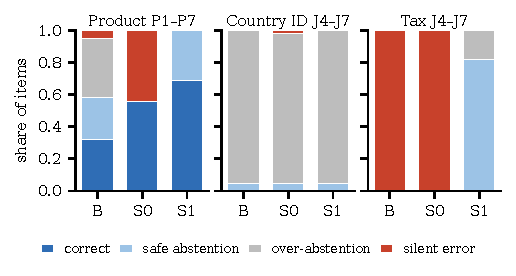
\includegraphics[width=\columnwidth]{figures/test_outcomes.pdf}
\caption{Outcome composition on TEST for the three pooled scopes ($n=359$, 769 and 769 items; Table~\ref{tab:primary}).
Explicit failures did not occur.}
\label{fig:outcomes}
\end{figure}

\subsection{Product Resolution: Coverage versus Silent Errors}
S0 answers every product item and is silently wrong on 159 of 359
(44.3\%): every under-specified, ambiguous and out-of-catalogue item receives an answer, and for 120 items S0 outputs its
hard-coded fallback code 8471.30 (four of these coincide with the true code). B answers far less (coverage 0.376) and has few silent errors (0.053, all on P4 and P6), but over-abstains on
every typo and confusable item. S1 answers 68.8\% [60.7, 75.1] with no silent error and a single over-abstention, on a
confusable item. Its decision accuracy (0.997 [0.991, 1.000]) is significantly higher than both B's and S0's
(Table~\ref{tab:tests}). Notably, the original pipeline S0 is \emph{not} more accurate than the baseline B
($-0.022$, Holm $p=1$); it trades B's over-abstention for silent errors. Table~\ref{tab:prodcat} shows that S1's coverage
loss is confined to items whose gold decision is decline (P4, P6, P7), plus one P5 item. On P8, S1 and B both abstain
on all 170 formal HS descriptions (24 of which name in-catalogue codes, hence over-abstentions), whereas S0 is silently
wrong on 167.

\begin{table}[t]
\centering
\caption{Product resolution on TEST by category: silent-error rate / coverage. Small categories (P4--P6) are descriptive only.}
\label{tab:prodcat}
\footnotesize
\setlength{\tabcolsep}{4pt}
\begin{tabular}{@{}lrccc@{}}
\toprule
Category & $n$ & B & S0 & S1 \\
\midrule
P1 & 76 & 0.000 / 1.000 & 0.000 / 1.000 & 0.000 / 1.000 \\
P2 & 75 & 0.000 / 0.533 & 0.093 / 1.000 & 0.000 / 1.000 \\
P3 & 75 & 0.000 / 0.000 & 0.453 / 1.000 & 0.000 / 1.000 \\
P4 & 15 & 1.000 / 1.000 & 1.000 / 1.000 & 0.000 / 0.000 \\
P5 & 22 & 0.000 / 0.000 & 0.318 / 1.000 & 0.000 / 0.955 \\
P6 & 10 & 0.400 / 0.400 & 1.000 / 1.000 & 0.000 / 0.000 \\
P7 & 86 & 0.000 / 0.000 & 1.000 / 1.000 & 0.000 / 0.000 \\
P8 & 170 & 0.000 / 0.000 & 0.982 / 1.000 & 0.000 / 0.000 \\
\bottomrule
\end{tabular}
\end{table}


\subsection{Country Identification and Tax Behaviour}
No system identified any held-out typo (J4) or
localised name (J5) correctly, apart from three J5 items for S0, which also produced 12 silent identification errors
(rate 0.016 [0.005, 0.029]). S1 and B abstain on all 734 J4/J5 items; their decision accuracy of 0.046 comes only from the
no-country categories J6 and J7. None of the six identification comparisons is significant after Holm correction. S1's
alias table identifies every in-table form (J1--J3, 696 items), but these are excluded from pooled claims by design. S1's
safety on held-out forms is therefore a product of abstention, not of better identification.

For tax behaviour, S1's result is achieved by refusal. B and S0 compute a landed cost for every held-out destination
and are silently wrong on 769 and 766 of 769 items. S1 computes no cost for any held-out form: it correctly refuses 632
items whose true jurisdiction has no rates, and over-refuses 137 (17.8\%) whose jurisdiction does have rates but whose
name it could not identify. Its decision accuracy (0.822 [0.755, 0.883]) and zero silent-error rate are thus achieved
entirely through refusal.

\begin{table}[t]
\centering
\caption{The 18 primary paired comparisons on TEST: difference (B$-$A) in the rate of the named outcome [95\% cluster-bootstrap interval] and Holm-adjusted cluster-level sign-flip permutation $p$ (10{,}000 permutations; minimum attainable 0.0018). DC = decision correct, SE = silent error.}
\label{tab:tests}
\footnotesize
\setlength{\tabcolsep}{2.5pt}
\begin{tabular}{@{}llllr@{}}
\toprule
Task & A$\rightarrow$B & Metric & Difference & Holm $p$ \\
\midrule
Product & B$\rightarrow$S0 & DC & $-0.022$ [$-0.142$, $+0.071$] & 1.00 \\
Product & B$\rightarrow$S0 & SE & $+0.390$ [$+0.327$, $+0.470$] & \textbf{0.0018} \\
Product & S0$\rightarrow$S1 & DC & $+0.440$ [$+0.381$, $+0.513$] & \textbf{0.0018} \\
Product & S0$\rightarrow$S1 & SE & $-0.443$ [$-0.515$, $-0.384$] & \textbf{0.0018} \\
Product & B$\rightarrow$S1 & DC & $+0.418$ [$+0.365$, $+0.459$] & \textbf{0.0018} \\
Product & B$\rightarrow$S1 & SE & $-0.053$ [$-0.071$, $-0.034$] & \textbf{0.0018} \\
\midrule
Ident. & B$\rightarrow$S0 & DC & $-0.003$ [$-0.010$, $+0.004$] & 1.00 \\
Ident. & B$\rightarrow$S0 & SE & $+0.016$ [$+0.005$, $+0.029$] & 0.0703 \\
Ident. & S0$\rightarrow$S1 & DC & $+0.003$ [$-0.004$, $+0.010$] & 1.00 \\
Ident. & S0$\rightarrow$S1 & SE & $-0.016$ [$-0.029$, $-0.005$] & 0.0703 \\
Ident. & B$\rightarrow$S1 & DC & $+0.000$ [$+0.000$, $+0.000$] & 1.00 \\
Ident. & B$\rightarrow$S1 & SE & $+0.000$ [$+0.000$, $+0.000$] & 1.00 \\
\midrule
Tax & B$\rightarrow$S0 & DC & $+0.004$ [$+0.000$, $+0.009$] & 1.00 \\
Tax & B$\rightarrow$S0 & SE & $-0.004$ [$-0.009$, $+0.000$] & 1.00 \\
Tax & S0$\rightarrow$S1 & DC & $+0.818$ [$+0.751$, $+0.880$] & \textbf{0.0018} \\
Tax & S0$\rightarrow$S1 & SE & $-0.996$ [$-1.000$, $-0.991$] & \textbf{0.0018} \\
Tax & B$\rightarrow$S1 & DC & $+0.822$ [$+0.757$, $+0.884$] & \textbf{0.0018} \\
Tax & B$\rightarrow$S1 & SE & $-1.000$ [$-1.000$, $-1.000$] & \textbf{0.0018} \\
\bottomrule
\end{tabular}
\end{table}


\subsection{Error Propagation and Malformed Inputs}
Table~\ref{tab:prop} separates the two controlled variations; within each block its classes are
mutually exclusive. Product errors never altered
duty, VAT or the landed cost for any system: the prototype's tax table assigns rates per country only, so a wrong code, including S0's fallback code, leaves the cost unchanged and surfaces instead as a wrong classification (and, for S0, a wrong
policy record on 14 items). Country errors did propagate: B and S0 produced silent landed-cost errors on 137 and 134
items, all computed with the default 5\%/10\% rates, with a median relative error of 10.3\% (maximum 13.75\%), and both
computed costs for all 632 items that should have been refused. The absence of cost errors from product mistakes is a
property of this prototype's tables, not evidence that product errors are harmless; with HS-dependent tariffs they
would propagate.

\begin{table}[t]
\centering
\caption{Error propagation on TEST and malformed-input handling. Within each block the classes are mutually exclusive and sum to $n$; classes that are zero for all systems are omitted, except the product landed-cost row. The fallback-code row is an overlapping attribute, not a class.}
\label{tab:prop}
\footnotesize
\setlength{\tabcolsep}{3pt}
\begin{tabular}{@{}lrrr@{}}
\toprule
Outcome class & B & S0 & S1 \\
\midrule
\multicolumn{4}{@{}l}{\emph{Product varied, country fixed (P1--P7, $n=359$)}} \\
No error & 116 & 200 & 247 \\
Product wrong or unresolved, flagged; cost unchanged & 132 & 0 & 0 \\
Product wrong, silent; cost unchanged & 0 & 48 & 0 \\
Landed-cost error & 0 & 0 & 0 \\
Should decline, cost computed, flagged & 92 & 0 & 0 \\
Should decline, cost computed, silent & 19 & 111 & 0 \\
Correct refusal & 0 & 0 & 111 \\
Over-refusal & 0 & 0 & 1 \\
Total & 359 & 359 & 359 \\
\quad\emph{Overlap:} S0 fallback code 8471.30$^\ast$ & 0 & 120 & 0 \\
\midrule
\multicolumn{4}{@{}l}{\emph{Country varied, product fixed (J4--J7, $n=769$)}} \\
No error & 0 & 3 & 0 \\
Landed-cost error, silent & 137 & 134 & 0 \\
Should refuse, cost computed, silent & 632 & 632 & 0 \\
Correct refusal & 0 & 0 & 632 \\
Over-refusal & 0 & 0 & 137 \\
Total & 769 & 769 & 769 \\
\midrule
\multicolumn{4}{@{}l}{\emph{Malformed inputs ($n=18$; not held out)}} \\
Rejected & 5 & 7 & 18 \\
Landed cost computed & 13 & 11 & 0 \\
\bottomrule
\end{tabular}
\\[2pt]\parbox{\columnwidth}{\scriptsize $^\ast$Items for which S0 output its hard-coded fallback HS code; they fall in three classes above: 83 \emph{should decline, silent}, 33 \emph{product wrong, silent} and 4 \emph{no error} (the fallback coincides with the true code of those items).}
\end{table}


S1 rejected all 18 malformed inputs. B and S0 rejected 5 and 7 and computed
landed costs for the rest, including negative, infinite and undefined (NaN) values. These 18 items are not split and
were also seen in the DEV stage, so this result is descriptive.

\subsection{Sensitivity, Exploratory and DEV Analyses}
Removing the sibling clusters of the eight excluded pilot items leaves the same nine tests
significant and S1's pooled product silent-error rate at zero.

Table~\ref{tab:ladder} adds one change at a time from S0 to S1 and ablates individual
components; these comparisons form a separate, exploratory family and are not confirmatory. Product gains appear when
product abstention is added (silent-error rate 0.443 $\rightarrow$ 0.120) and when the evidence tiers are added
($\rightarrow$ 0.000); the tax-behaviour gain appears entirely at the refusal step. Removing S1's typo tier reduces
product coverage to 0.454; removing the coverage guard yields one silent error on P1--P7 and 13 on P8, although the
threshold had no effect on DEV. Adding country typo matching, which was not part of the pre-declared S1, raises held-out
identification accuracy to 0.397 without silent errors; whether it generalises would require a new held-out evaluation.

\begin{table}[t]
\centering
\caption{\emph{Exploratory} attribution ladder and ablations on TEST (pooled scopes): decision accuracy / silent-error rate. Not part of the confirmatory family.}
\label{tab:ladder}
\footnotesize
\setlength{\tabcolsep}{3pt}
\begin{tabular}{@{}lccc@{}}
\toprule
Variant & Product & Ident. & Tax \\
\midrule
L0 = S0 & 0.557 / 0.443 & 0.043 / 0.016 & 0.004 / 0.996 \\
L1 +validation & 0.557 / 0.443 & 0.043 / 0.016 & 0.004 / 0.996 \\
L2 +ISO identification & 0.557 / 0.443 & 0.046 / 0.000 & 0.000 / 1.000 \\
L3 +refuse w/o tax data & 0.557 / 0.443 & 0.046 / 0.000 & 0.822 / 0.000 \\
L4 +product abstention & 0.777 / 0.120 & 0.046 / 0.000 & 0.822 / 0.000 \\
L5 +evidence tiers = S1 & 0.997 / 0.000 & 0.046 / 0.000 & 0.822 / 0.000 \\
\midrule
S1 $-$typo tier & 0.763 / 0.000 & 0.046 / 0.000 & 0.822 / 0.000 \\
S1 $-$coverage guard & 0.994 / 0.003 & 0.046 / 0.000 & 0.822 / 0.000 \\
S1 +country typo & 0.997 / 0.000 & 0.397 / 0.000 & 0.878 / 0.000 \\
S0 $-$token overlap & 0.343 / 0.657 & 0.043 / 0.016 & 0.004 / 0.996 \\
S0 $-$partial country & 0.557 / 0.443 & 0.046 / 0.000 & 0.000 / 1.000 \\
\bottomrule
\end{tabular}
\end{table}


On DEV, where S1 was tuned, its pooled product decision accuracy was 1.000 with coverage
0.773; on TEST, 0.997 with coverage 0.688. The difference in coverage partly reflects category mix (out-of-catalogue
items are 25 of 198 DEV items but 86 of 359 TEST items). DEV latency was indicative only: median per-call times of 0.149,
2.108 and 0.671\,ms (B, S0, S1) on the product workload, measured on a shared cloud machine; TEST was never timed.

\section{Threats to Validity}
The catalogue, perturbations, tax rates and policy records are synthetic or unsourced;
``correct'' means correct with respect to the project's own tables. The HS texts come from an unofficial mirror with
abridged descriptions, and the catalogue's HS assignments are unverified. Nothing here establishes legal classification
validity, regulatory compliance or production readiness.

Construct and external validity are limited because benchmark categories were constructed by rule; real trader input may differ.
The results cover 60 product types and 40 jurisdictions. Because tariffs in the prototype do not depend on the HS code,
the propagation result for products does not transfer to real tariff schedules.

For internal validity, the main threat is that the same team, with AI assistance, designed the systems, the benchmark and the evaluation.
Labels never derive from system outputs, the data and code were frozen before TEST, and TEST was evaluated once, but
same-team design remains a threat. The pilot had a single reviewer. S1's tuning selected among seven DEV-tied settings
by a pre-declared tie-break.

Regarding statistical conclusion validity, several categories have few clusters; intervals there are wide or degenerate
and are not interpreted. Holm correction covers the 18 primary tests; exploratory comparisons are corrected only within
their own family.

\section{Conclusion}
In this prototype, making abstention explicit removed silent errors where the input could not be resolved: on held-out
products S1 made no silent error while answering about two thirds of items, and the original six-stage pipeline was no
more accurate than a single-step baseline while being silently wrong on 44\% of items. The gains are uneven. No system
reliably identifies held-out country forms, and S1's tax-data safety is achieved by refusing, including 137 refusals where
rates existed. The propagation analysis shows that silent jurisdiction defaults, not product errors, drove the
financial errors in this prototype, because its rates depend on the country alone. Future work should extend
jurisdiction identification to localised and misspelt names and evaluate it on a new held-out split, use HS-dependent
tariffs, and test with real, consented trader descriptions.

\section*{Acknowledgment}
An AI assistant (Claude, Anthropic, used through Claude Code) was used extensively in this
work: analysing the original repository; supporting research planning and the evaluation design; writing the S1 code,
the benchmark generators, the evaluation, statistics and run-control code and their tests; executing the authorised
build, freeze, tuning, DEV and TEST stages; searching for and verifying literature metadata; and drafting this
manuscript, including its tables and figure. The authors defined the research question and scope, made the review,
exclusion, freeze and evaluation decisions, and are responsible for all content.

\bibliographystyle{IEEEtran}
\bibliography{references}

\end{document}
